\documentclass{lab_sheet}
\usepackage{nccmath}
\usepackage{tikz}
\usetikzlibrary{arrows}
\usepackage{hyperref}
\newcommand\ddfrac[2]{\frac{\displaystyle #1}{\displaystyle #2}}
\newcommand{\proteusObservationA}[4]{ 
\begin{figure}[H]
   \begin{minipage}[b]{0.60\linewidth}
     \centering
     \includegraphics[width=\linewidth]{../Figures/#1.PDF}
   \end{minipage}%
   \begin{minipage}[b]{0.40\linewidth}
     \centering
 \begin{tabular}[b]{|M{4cm}|M{1cm}|}
   \hline
   \multicolumn{2}{|c|}{Noted Values} \\
   \hline \hline
   DC gain (in dB) & #2\\ \hline
   Half power frequency (in KHz) & #3\\ \hline
 \end{tabular}
 \end{minipage}
 \caption{Observation for #4}
 \label{fig:prot_obs_a_#1}
 \end{figure}
}
\newcommand{\proteusObservationB}[4]{ 
\begin{figure}[H]
   \begin{minipage}[b]{0.60\linewidth}
     \centering
     \includegraphics[width=\linewidth]{../Figures/#1.PDF}
   \end{minipage}%
   \begin{minipage}[b]{0.40\linewidth}
     \centering
 \begin{tabular}[b]{|M{4cm}|M{1cm}|}
   \hline
   \multicolumn{2}{|c|}{Noted Values} \\
   \hline \hline
   Gain in passband (in dB) & #2\\ \hline
   Half power frequency (in KHz) & #3\\ \hline
 \end{tabular}
 \end{minipage}
 \caption{Observation for #4}
 \label{fig:prot_obs_a_#1}
 \end{figure}
}
\newcommand{\figgic}{
    \begin{circuitikz}[american,scale = 0.93, transform shape]   
        \draw
        (1.5,0) node [op amp, noinv input up] (opamp1) {}
        (-6,-2) to [generic,l=$Z_1$,*-*] (-3,-2) to [generic,l=$Z_2$,-*] (0,-2) to [generic,l=$Z_3$,-*] (3,-2) to [generic,l=$Z_4$,-*] (6,-2) to [generic,l=$Z_5$] (8,-2) node [right] {$V_2$} to [short] (8,-4) node [ground]{}
        (-1.5,-4) node [op amp, noinv input up,rotate=180] (opamp2) {}
        (-7,-2) node [left] {$V_{1}$} to [short,o-]  (-6,-2) |- (opamp1.+)
        (6,-2) |- (opamp2.+)
        (-3,-2) |- (opamp2.out)
        (3,-2) |- (opamp1.out)
        (0,-2) |- (opamp1.-)
        (0,-2) |- (opamp2.-)
        (-7,-3) node [left] {$Z_{in}$} 
        (-7,-3.5) to [short,o-] (-7,-4) node[ground] {}
        ;
        \draw[->,thick](-7,-3) -- (-6,-3);
            \end{circuitikz}
}

\newcommand{\figquestion}{
   \begin{circuitikz}[american]
      \draw
      (0,0) to[R,l= \footnotesize$R_1\text{ = }1\text{ }\Omega$] (2,0) to [L,l=\footnotesize$L_1\text{ = }0.7654\text{ H}$] (4,0) to [C, *-*, l_=\footnotesize$C_1\text{ = }1.848 \text{ F}$] (4,-4)
      (4,0) to [L,l=\footnotesize$L_2\text{ = }1.848\text{ H}$] (8,0) to [C, *-*, l_=\footnotesize$C_2\text{ = }0.7654 \text{ F}$] (8,-4)
      (8,0) to [short] (12,0)
      (0,0) to [esource,v_=\footnotesize$V_1$] (0,-4)
      (0,-4) to [short] (12,-4) to[R, l=\footnotesize$R_2\text{ = }1\Omega$, v<=\footnotesize$V_2$] (12,0)
         ;
      \end{circuitikz}
}

\newcommand{\figleap}{
   \begin{circuitikz}[american]
      \draw
      (0,0) to[generic,l= \footnotesize$Z_1\text{ = }1+0.7654s$,i_=\footnotesize$I_1$] (4,0) to [generic, *-*, l_=\footnotesize$Z_2\text{ = }\ddfrac{1}{1.848s}$] (4,-4)
      (4,0) node (v3) [anchor=south] {\footnotesize$V_3$} to [generic,l=\footnotesize$Z_3\text{ = }1.848s$,i_=\footnotesize$I_2$] (8,0) (8,-4) to [generic, l=\footnotesize$Z_4\text{ = }\ddfrac{1}{1+0.7654s}$,*-*] (8,0) node (v4) [anchor=south] {\footnotesize$V_4$} to [short,-o] (9,0)
      (8,-4) to [short,-o] (9,-4)
      (0,0) to [esource,v_=\footnotesize$V_1$] (0,-4)
      (9,0) to [open,v_=\footnotesize$V_2$] (9,-4)
      (0,-4) to [short] (8,-4) 
         ;
      \end{circuitikz}
}

\newcommand{\figfdnr}{
   \begin{circuitikz}[american]
      \draw
      (0,0) to[C,l= \footnotesize$Z'_{R\textsubscript{$1$}}\text{ = }1\text{ F}$] (2,0) to [R,l=\footnotesize$Z'_{L\textsubscript{$1$}}\text{ = }0.7654\text{ }\Omega$] (4,0)  to [R,l=\footnotesize$Z'_{L\textsubscript{$2$}}\text{ = }1.848\text{ }\Omega$] (8,0) to [short] (12,0)
      (0,0) to [esource,v_=\footnotesize$V_1$] (0,-4)
      (0,-4) to [short] (12,-4) to[C, l=\footnotesize$Z'_{R\textsubscript{$2$}}\text{ = }1\text{ F}$, v<=\footnotesize$V_2$] (12,0)
      (4,0) to [short,*-] (4,-1.6)
      (4,-2.2) to [short,-*] (4,-4)
      (3.7,-2) node [left] {\footnotesize$Z'_{C\textsubscript{$1$}}\text{ = }1.848$} 
      (8,0) to [short,*-] (8,-1.6)
      (8,-2.2) to [short,-*] (8,-4)
      (7.7,-2) node [left] {\footnotesize$Z'_{C\textsubscript{$2$}}\text{ = }0.7654$} 
         ;
       \draw [thick] (3.7,-1.6)-- (4.3,-1.6);
       \draw [thick] (3.7,-1.8)-- (4.3,-1.8);
       \draw [thick] (3.7,-2)-- (4.3,-2);
       \draw [thick] (3.7,-2.2)-- (4.3,-2.2);

       \draw [thick] (7.7,-1.6)-- (8.3,-1.6);
       \draw [thick] (7.7,-1.8)-- (8.3,-1.8);
       \draw [thick] (7.7,-2)-- (8.3,-2);
       \draw [thick] (7.7,-2.2)-- (8.3,-2.2);
       
      \end{circuitikz}
}


\newcommand{\fighp}{
   \begin{circuitikz}[american]
      \draw
      (0,0) to[R,l= \footnotesize$Z'_{R\textsubscript{$1$}}\text{ = }1\text{ }\Omega$] (2,0) to [C,l=\footnotesize$Z'_{L\textsubscript{$1$}}\text{ = }1.3065\text{ F}$] (4,0) to [L,l_=\footnotesize$Z'_{C\textsubscript{$1$}}\text{ = }0.5411\text{ H}$, *-*] (4,-4) (4,0) to [C,l=\footnotesize$Z'_{L\textsubscript{$2$}}\text{ = }0.5411\text{ F}$] (8,0) to [L,l_=\footnotesize$Z'_{C\textsubscript{$2$}}\text{ = }1.3065\text{ H}$, *-*] (8,-4) 
      (8,0) to [short] (12,0)
      (0,0) to [esource,v_=\footnotesize$V_1$] (0,-4)
      (0,-4) to [short] (12,-4) to[R, l=\footnotesize$Z'_{R\textsubscript{$2$}}\text{ = }1\text{ }\Omega$, v<=\footnotesize$V_2$] (12,0)
         ;
      \end{circuitikz}
}

\newcommand{\figla}{
    \begin{circuitikz}[american,scale = 0.9, transform shape]
    \draw
    (0,0) node [op amp] (opamp) {}
    (5,-0.5) node [op amp] (opamp2) {}
    (-4,1) node [left] {$V_1$} to [R, l=$1\text{ }\Omega$, o-] (-2,1) to [short] (-2,0)
    to [R, l_=$1\text{ }\Omega$, -o] (-4,0) node [left] {$-V_3$}
    (-2,0.5) to [short,*-*] (opamp.-) |- (-0.75,2.25) to[short,*-] (-1.2,2.25)
    (-0.75,3) to [C,l=$0.7654\text{ F}$] (0.75,3) to[short] (0.75,1.75) to [R,l_=$1\text{ }\Omega$] (-0.75, 1.75) to [short] (-0.75,3)
    (0.75,2.25) to[short,*-] (1.2,2.25) -| (opamp.out) to [R,*-*,l=$1\text{ }\Omega$] (opamp2.-)
    |- (4,1) to [short][R,l=$1\text{ }\Omega$]  (6,1) -| (opamp2.out) to [short,*-o] (7,-0.5) node [right] {$V_{I1}$}
    (opamp.+) node[ground] {}
    (opamp2.+) node[ground] {}
    ;
        \end{circuitikz}
}

\newcommand{\figlb}{
    \begin{circuitikz}[american,scale = 0.9, transform shape]
    \draw
    (0,0) node [op amp] (opamp) {}
    (-4,1) node [left] {$V_{I1}$} to [R, l=$1\text{ }\Omega$, o-] (-2,1) to [short] (-2,0)
    to [R, l_=$1\text{ }\Omega$, -o] (-4,0) node [left] {$-V_{I2}$}
    (-2,0.5) to [short,*-*] (opamp.-) |- (-0.75,1.5) to [C,l=$1.848\text{ F}$] (0.75,1.5) -| (opamp.out) to [short,*-o] (2.2,0) node [right] {$-V_{3}$}
    (opamp.+) node[ground] {}
    ;
        \end{circuitikz}
}

\newcommand{\figlc}{
    \begin{circuitikz}[american,scale = 0.9, transform shape]
    \draw
    (0,0) node [op amp] (opamp) {}
    (5,-0.5) node [op amp] (opamp2) {}
    (-4,1) node [left] {$V_{4}$} to [R, l=$1\text{ }\Omega$, o-] (-2,1) to [short] (-2,0)
    to [R, l_=$1\text{ }\Omega$, -o] (-4,0) node [left] {$-V_{3}$}
    (-2,0.5) to [short,*-*] (opamp.-) |- (-0.75,1.5) to [C,l=$1.848\text{ F}$] (0.75,1.5) -| (opamp.out) to [R,*-*,l=$1\text{ }\Omega$] (opamp2.-) |- (4,1) to [short][R,l=$1\text{ }\Omega$]  (6,1) -| (opamp2.out) to [short,*-o] (7,-0.5) node [right] {$-V_{I2}$}
    (opamp.+) node[ground] {}
    (opamp2.+) node[ground] {}
    ;
        \end{circuitikz}
}

\newcommand{\figld}{
    \begin{circuitikz}[american,scale = 0.9, transform shape]
    \draw
    (0,0) node [op amp] (opamp) {}
    (-4,0.5) node [left] {$-V_{I2}$} to [R, l=$1\text{ }\Omega$, o-*] (opamp.-) |- (-0.75,2.25) to[short,*-] (-1.2,2.25)
    (-0.75,3) to [C,l=$0.7654\text{ F}$] (0.75,3) to[short] (0.75,1.75) to [R,l_=$1\text{ }\Omega$] (-0.75, 1.75) to [short] (-0.75,3)
    (0.75,2.25) to[short,*-] (1.2,2.25) -| (opamp.out) to [short,*-o] (2.2,0) node [right] {$V_4$}
    (opamp.+) node[ground] {}
    ;
        \end{circuitikz}
}

\begin{document}
    \titlePage{Design of Higher Order Active Filter using Active Simulation of Passive Filters}{August 11, 2021}
    \pagenumbering{roman}
    \clearpage
    \tableofcontents
    \clearpage
    \phantomsection
    \addcontentsline{toc}{section}{\bfseries{List of Figures}}
    \listoffigures
    \clearpage
    \pagenumbering{arabic}
    \section{Objectives}
    \begin{itemize}
        \item To be familiar with the design of higher order active filters using simulated inductors.
        \item To be familiar with the design of higher order active filters using Frequency Dependent Negative Resistor (FDNR).
        \item To be familiar with the design of higher order active filters using leapfrog simulation.
    \end{itemize}
    \section{Background Theory}
    \subsection{Design of higher order active filters}
    The design of higher order active filters can be performed by two methods,
    \begin{enumerate}
        \item Cascade of biquad circuits
        \item Active simulation of passive filters
        \begin{enumerate}
            \item Elemental simulation
            \begin{itemize}
                \item Ladder design with simulated inductors
                \item Ladder design with Frequency Dependent Negative Resistor (FDNR)
            \end{itemize}
            \item Functional simulation
            \begin{itemize}
                \item Leapfrog simulation of ladders
            \end{itemize}
        \end{enumerate}
    \end{enumerate}
    \subsubsection{Cascade of biqaud circuits}
    For a higher order active filter with transfer function $T(s)$, the realization is possible as the ratio of the output voltage to input voltage of a cascade connection of lower order stages that don't cause load effect. For this to be possible, the output impedance of each stage needs to be lower than the input impedance of the following stage at all interested frequencies. This is possible since op-amps offer high input impedance and low output impedance.
    If $T(s)$ is the required transfer function given as,
    \begin{equation*}
        T(s)=\frac{a_ms^m+a_{m-1}s^{m-1}+\cdots+a_0}{s^n+b_{n-1}s^{n-1}+\cdots+b_0}
    \end{equation*}
    For $n$ as even, $T(s)$ is expressed as,
    \begin{equation*} 
            T(s)=\prod_{i=1}^{\frac{n}{2}}\frac{a_{2i}s^2+a_{1i}s+a_{0i}}{s^2+b_{1i}s+b_{0i}}=\prod_{i=1}^{\frac{n}{2}}T_i(s)
    \end{equation*}
    For $n$ as odd, $T(s)$ is expressed as,
    \begin{equation*} 
      \begin{aligned}
          T(s)=\frac{a_{11}s+a_{01}}{s+b_{01}}\prod_{i=2}^{\frac{n-1}{2}}\frac{a_{2i}s^2+a_{1i}s+a_{0i}}{s^2+b_{1i}s+b_{0i}}=T_1(s)\prod_{i=2}^{\frac{n-1}{2}}T_i(s)
      \end{aligned}
\end{equation*}
    \subsubsection{Active simulation of passive filters}
    This method of designing higher order active filters is based on the simulation of passive filters using some active components. For a readily available passive circuit, the active simulation is much more easier than designing using cascading. A Generalized Impedance Converter (GIC), a two port network that is primarily used to convert one form of impedance into another is a major component in designing higher order active filters using active simulation of passive filters.

    \begin{figure}[H]
        \centering
        \figgic
        \caption{Antoniou's Generalized Impedance Converter (GIC)}
        \label{fig:gic}
    \end{figure}
    The impedance $Z_{in}$ from the input side is given as,
    \begin{equation}
        Z_{in}=\frac{Z_1Z_3Z_5}{Z_2Z_4}
        \label{eqn:gic}
    \end{equation}
    \subsubsubsection{Ladder design with simulated inductor}
    This method is a form of elemental simulation using a GIC, where a grounded inductor in a passive circuit is replaced with a GIC to convert the passive circuit into active. For Figure~\ref{fig:gic}, if $Z_1=Z_2=Z_3=1$ $\Omega$, $Z_4=1$ F and $Z_5=k$ $\Omega$, then from Equation~\ref{eqn:gic}, we get,
    \begin{equation*}
        Z_{in}=\ddfrac{1\times1\times k}{\left(\frac{1}{s}\right)\times1}=ks
    \end{equation*}

    \subsubsubsection{Ladder design with Frequency Dependent Negative Resistor (FDNR)}
    This method is also a form of elemental simulation where a magnitude scaling factor of $K_m=\ddfrac{1}{s}$ is used, that ultimately converts a resistor to a capacitor $\left(\ddfrac{R}{s}\right)$, an inductor a resistor $(L)$, and the capacitor to a Frequency Dependent Negative Resistor (FDNR) $\left(\ddfrac{1}{s^2C}\right)$. To realize the FDNR, a GIC shown in Figure~\ref{fig:gic} with $Z_1=Z_2=1$ $\Omega$, $Z_3=Z_5=1$ F and $Z_4=k$ $\Omega$ is used. So, from Equation~\ref{eqn:gic}, we get,
    \begin{equation*}
            Z_{in}=\ddfrac{\left(\frac{1}{s}\right)\times\left(\frac{1}{s}\right)\times 1}{1\times k}=\frac{1}{ks^2} 
    \end{equation*}
    \subsubsubsection{Leapfrog simulation of ladders}
    This method is a form of functional simulation to design higher order active filters from passive filters. In this method, each component in the passive circuit is initially replaced by an equivalent impedance or admittance and admittance or impedance groups are created based on same cur­rent (series) or same voltage (parallel) configuration giving rise to a block diagram equivalent to the original circuit. Each block is then implemented either by using an inverting summer (for summing blocks) or active circuits (for admittance and impedance blocks) to complete the active simulation of the passive filter.
    \section{Exercises}
    \begin{figure}[H]
        \centering
        \figquestion
        \caption{Fourth order butterworth lowpass ladder circuit at 1 rad/s}
        \label{fig:ques}
    \end{figure}
    \mysub{Design of higher order active filters using FDNR}
    \problem{The network given in Figure~\ref{fig:ques} is the fourth order Butterworth lowpass filter at normalized frequency of 1 rad/sec. From this network, design a lowpass filter having half power frequency of 20000 rad/sec using FDNR. Realize the network and observe the magnitude response.}
    Using Bruton's transformation on the circuit shown in Figure~\ref{fig:ques}, i.e. using magnitude scaling factor of $K_m=\ddfrac{1}{s}$, we get the conversions as,
    \begin{equation*}
        \begin{aligned}
           & Z'_{R\textsubscript{$1$}}=1 \text{ F} \quad && Z'_{R\textsubscript{$2$}}=1 \text{ F}\\
           & Z'_{L\textsubscript{$1$}}=0.7654 \text{ }\Omega \quad && Z'_{L\textsubscript{$2$}}=1.848 \text{ }\Omega\\
           & Z'_{C\textsubscript{$1$}}=1.848 \text{ (FDNR)} \quad && Z'_{C\textsubscript{$2$}}=0.7654 \text{ (FDNR)}\\
        \end{aligned}
    \end{equation*}
    The resulting circuit with FDNR is given as, 
    \begin{figure}[H]
        \centering
        \figfdnr
        \caption{Fourth order butterworth lowpass ladder circuit using FDNR}
        \label{fig:fdnr}
    \end{figure}
    To realize FDNR $Z'_{C\textsubscript{$1$}}$ a GIC shown in Figure~\ref{fig:gic} is used. For $Z_1=Z_2=1$ $\Omega$, $Z_3=Z_5=1$ F and $Z_4=k$ $\Omega$, from Equation~\ref{eqn:gic}, we get,
    \begin{equation*}
        \begin{aligned}
            Z_{in}&=Z'_{C\textsubscript{$1$}}=\ddfrac{1\times\left(\frac{1}{s}\right)\times\left(\frac{1}{s}\right)}{1\times k}\\
            &\Rightarrow \frac{1}{1.848s^2}=\frac{1}{ks^2}\\
            &\therefore k=1.848 \text{ }\Omega
        \end{aligned}
    \end{equation*}
    To realize FDNR $Z'_{C\textsubscript{$2$}}$ a GIC shown in Figure~\ref{fig:gic} is used. For $Z_1=Z_2=1$ $\Omega$, $Z_3=Z_5=1$ F and $Z_4=k$ $\Omega$, from Equation~\ref{eqn:gic}, we get,
    \begin{equation*}
        \begin{aligned}
            Z_{in}&=Z'_{C\textsubscript{$2$}}=\ddfrac{1\times\left(\frac{1}{s}\right)\times\left(\frac{1}{s}\right)}{1\times k}\\
            &\Rightarrow \frac{1}{0.7654s^2}=\frac{1}{ks^2}\\
            &\therefore k=0.7654 \text{ }\Omega
        \end{aligned}
    \end{equation*}
    Since we require the lowpass filter having frequency of $20000$ rad/s, a frequency scaling factor of $K_f=\ddfrac{20000}{1}=2\times 10^4$ is used. Similarly, for practically realizable values, a magnitude scaling factor of $K_m=10^3$ is used.\\ The scaled components are,
    \begin{equation*}
        \begin{aligned}
           & Z'_{R\textsubscript{$1$}}=\frac{1}{2\times 10^4\times10^3}=50\text{ nF}\quad && Z'_{R\textsubscript{$2$}}=\frac{1}{2\times 10^4\times10^3}=50\text{ nF}\\
           & Z'_{L\textsubscript{$1$}}=0.7654\times10^3=765.4\text{ }\Omega \quad && Z'_{L\textsubscript{$2$}}=1.848\times10^3=1.848\text{ K}\Omega
        \end{aligned}
    \end{equation*}
    The impedances that are used in the GIC implementation of the two FNDRs $Z'_{C\textsubscript{$1$}}$ and $Z'_{C\textsubscript{$2$}}$ are also scaled as,\\
    \textbf{Scaled impedances required for implementing $Z'_{C\textsubscript{$1$}}$ using GIC}
    \begin{equation*}
        \begin{aligned}
            & Z_1=Z_2=1\times10^3=1\text{ K}\Omega \quad && Z_3=Z_5=\frac{1}{2\times10^4\times10^3}=50\text{ nF}\\
            &Z_4=1.848\times10^3=1.848\text{ K}\Omega
        \end{aligned}
    \end{equation*}
    \textbf{Scaled impedances required for implementing $Z'_{C\textsubscript{$2$}}$ using GIC}
    \begin{equation*}
        \begin{aligned}
            & Z_1=Z_2=1\times10^3=1\text{ K}\Omega \quad && Z_3=Z_5=\frac{1}{2\times10^4\times10^3}=50\text{ nF}\\
            &Z_4=0.7654\times10^3=765.4\text{ }\Omega
        \end{aligned}
    \end{equation*}
    \begin{figure}[H]
        \centering
        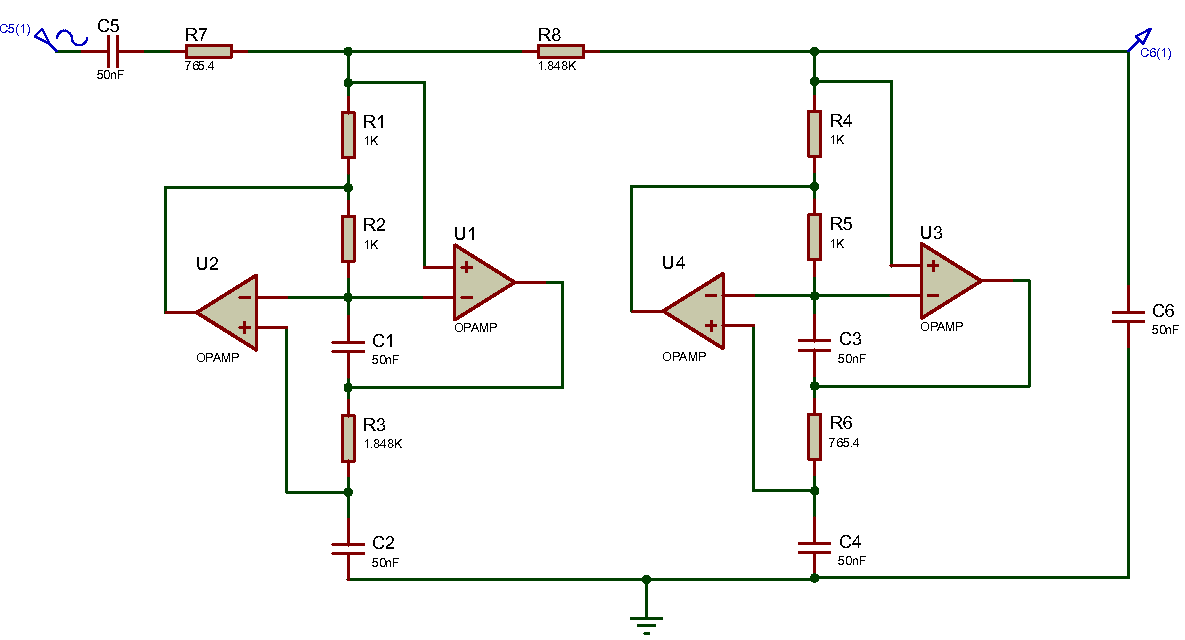
\includegraphics[width=\linewidth]{../Figures/ckt_a}
        \caption{Proteus circuit for designed lowpass filter at 20000 rad/s}
        \label{fig:protA}
    \end{figure}
    \proteusObservationA{protA}{-6.02}{3.177}{lowpass filter designed in Problem 1}


    \mysub{Design of higher order active filters using simulated inductor}
    \problem{Obtain a highpass filter at normalized frequency of 1 rad/sec from the lowpass filter given in Figure~\ref{fig:ques} using frequency transformation. From the circuit obtained, design a highpass filter using simulated inductors. In your final design the half power frequency should be 4775 Hz and practically realizable elements. Realize the filter network. Also observe and analyze the magnitude response of the filter network.}
Using frequency transformation on the circuit shown in Figure~\ref{fig:ques} to design a highpass filter at $1$ rad/s, we get the conversions as,
\begin{equation*}
    \begin{aligned}
       & Z'_{R\textsubscript{$1$}}=1 \text{ }\Omega \quad && Z'_{R\textsubscript{$2$}}=1 \text{ }\Omega\\
       & Z'_{L\textsubscript{$1$}}=1.3065 \text{ F} \quad && Z'_{L\textsubscript{$2$}}=0.5411 \text{ F}\\
       & Z'_{C\textsubscript{$1$}}=0.5411 \text{ H} \quad && Z'_{C\textsubscript{$2$}}=1.3065 \text{ H}\\
    \end{aligned}
\end{equation*}
The resulting highpass ladder circuit is given as,
\begin{figure}[H]
    \centering
    \fighp
    \caption{Fourth order butterworth highpass ladder circuit at 1 rad/s}
    \label{fig:hp}
\end{figure}

To simulate the inductor $Z'_{C\textsubscript{$1$}}$ a GIC shown in Figure~\ref{fig:gic} is used. For $Z_1=Z_2=Z_3=1$ $\Omega$, $Z_4=1$ F and $Z_5=k$ $\Omega$, from Equation~\ref{eqn:gic}, we get,
    \begin{equation*}
        \begin{aligned}
            Z_{in}&=Z'_{C\textsubscript{$1$}}=\ddfrac{1\times1\times k}{\left(\frac{1}{s}\right)\times 1}\\
            &\Rightarrow 0.5411s=s\times k\\
            &\therefore k=0.5411 \text{ }\Omega
        \end{aligned}
    \end{equation*}

    
To simulate the inductor $Z'_{C\textsubscript{$1$}}$ a GIC shown in Figure~\ref{fig:gic} is used. For $Z_1=Z_2=Z_3=1$ $\Omega$, $Z_4=1$ F and $Z_5=k$ $\Omega$, from Equation~\ref{eqn:gic}, we get,
\begin{equation*}
    \begin{aligned}
        Z_{in}&=Z'_{C\textsubscript{$2$}}=\ddfrac{1\times1\times k}{\left(\frac{1}{s}\right)\times 1}\\
        &\Rightarrow 1.3065s=s\times k\\
        &\therefore k=1.3065 \text{ }\Omega
    \end{aligned}
\end{equation*}
Since we require the highpass filter having frequency of $4775$ Hz, a frequency scaling factor of $K_f=\ddfrac{2\pi\times4775}{1}\approx 3\times 10^4$ is used. Similarly, for practically realizable values, a magnitude scaling factor of $K_m=10^3$ is used.\\ The scaled components are,
\begin{equation*}
    \begin{aligned}
       & Z'_{R\textsubscript{$1$}}=1\times10^3=1\text{ K}\Omega\quad && Z'_{R\textsubscript{$2$}}=1\times10^3=1\text{ K}\Omega\\
       & Z'_{L\textsubscript{$1$}}=\frac{1.3065}{3\times10^4\times10^3}=43.55\text{ nF} \quad && Z'_{L\textsubscript{$2$}}=\frac{0.5411}{3\times10^4\times10^3}=18.04\text{ nF} 
    \end{aligned}
\end{equation*}
The impedances that are used in the GIC implementation of the two inductors $Z'_{C\textsubscript{$1$}}$ and $Z'_{C\textsubscript{$2$}}$ are also scaled as,\\
\textbf{Scaled impedances required for implementing $Z'_{C\textsubscript{$1$}}$ using GIC}
\begin{equation*}
    \begin{aligned}
        & Z_1=Z_2=Z_3=1\times10^3=1\text{ K}\Omega \quad && Z_4=\frac{1}{3\times10^4\times10^3}=33.33\text{ nF}\\
        &Z_5=0.5411\times10^3=541.1\text{ }\Omega
    \end{aligned}
\end{equation*}
\textbf{Scaled impedances required for implementing $Z'_{C\textsubscript{$2$}}$ using GIC}
\begin{equation*}
    \begin{aligned}
        & Z_1=Z_2=Z_3=1\times10^3=1\text{ K}\Omega \quad && Z_4=\frac{1}{3\times10^4\times10^3}=33.33\text{ nF}\\
        &Z_5=1.3065\times10^3=1.3065\text{ K}\Omega
    \end{aligned}
\end{equation*}

\begin{figure}[H]
    \centering
    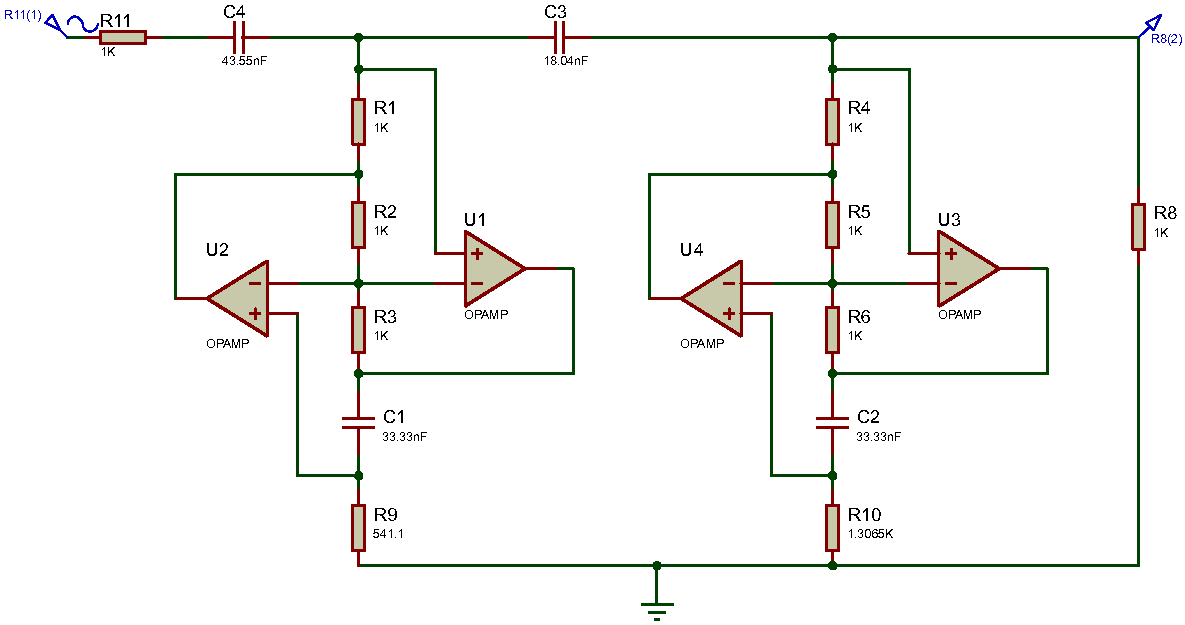
\includegraphics[width=\linewidth]{../Figures/ckt_b}
    \caption{Proteus circuit for designed highpass filter at 4775 Hz}
    \label{fig:protB}
\end{figure}

\proteusObservationB{protB}{-6.02}{4.86}{highpass filter designed in Problem 2}

\mysub{Design of higher order active filters using leapfrog simulation}
\problem{From the circuit given in Figure~\ref{fig:ques}, design a lowpass passive filter having half power frequency of 40000 rad/sec with practically suitable elements, using Leapfrog simulation. Realize the filter network and observe the magnitude response of the network.}
Representing Figure~\ref{fig:ques} as block diagrams of impedances as,
\begin{figure}[H]
    \centering
    \figleap
    \caption{Block diagram representation of the fourth order butterworth lowpass filter}
    \label{fig:leap}
\end{figure}
Applying voltage and nodal analysis for Figure~\ref{fig:leap}, we get,
\begin{equation}
    I_1=\frac{V_1-V_3}{Z_1}=T_1(V_1-V_3) \quad \text{where, } T_1=\frac{1}{Z_1}=\frac{1}{1+0.7654s}
    \label{eqn:leap-1}
\end{equation}
\begin{equation}
  V_3=Z_2(I_1-I_2)=T_2(I_1-I_2) \quad \text{where, } T_2=Z_2=\frac{1}{1.848s}
  \label{eqn:leap-2}
\end{equation}
\begin{equation}
    I_2=\frac{V_3-V_4}{Z_3}= T_3(V_3-V_4) \quad \text{where, }T_3=\frac{1}{Z_3}=\frac{1}{1.848s}
    \label{eqn:leap-3}
\end{equation}
\begin{equation}
    V_4=Z_4I_2=T_4I_2 \quad \text{where, }T_4=Z_4=\frac{1}{1+0.7654s}
    \label{eqn:leap-4}
\end{equation}
Let $V_{I1}=I_1$ and $V_{I2}=I_2$, we get, 
\begin{equation}
    V_{I1}=-(-T_1)(V_1-V_3)
    \label{eqn:leap-ar-1}
\end{equation}
\begin{equation}
    -V_3=-T_2(V_{I1}-V_{I2})
    \label{eqn:leap-ar-2}
\end{equation}
\begin{equation}
    -V_{I2}=-(-T_3)(V_4-V_3)
    \label{eqn:leap-ar-3}
\end{equation}
\begin{equation}
    V_4=(-T_4)(-V_{I2})
    \label{eqn:leap-ar-4}
\end{equation}
\begin{figure}[H]
    \centering
    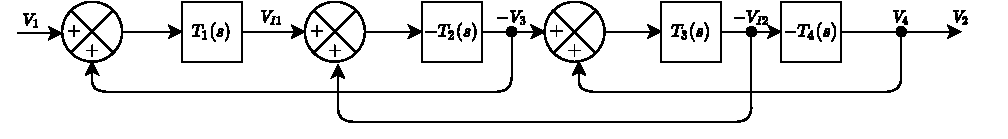
\includegraphics[width=\linewidth]{../Figures/leapfrog}
    \caption{Block diagram representation of circuit equations}
    \label{fig:leapfrog-block}
\end{figure}

Realization for Equation~\ref{eqn:leap-ar-1} is given as,

\begin{figure}[H]
    \centering
    \figla
    \caption{Realization of Equation~\ref{eqn:leap-ar-1}}
\end{figure}

\begin{figure}[H]
    \centering
    \figlb
    \caption{Realization of Equation~\ref{eqn:leap-ar-2}}
\end{figure}

\begin{figure}[H]
    \centering
    \figlc
    \caption{Realization of Equation~\ref{eqn:leap-ar-3}}
\end{figure}

\begin{figure}[H]
    \centering
    \figld
    \caption{Realization of Equation~\ref{eqn:leap-ar-4}}
\end{figure}
Since we require the lowpass filter having frequency of $40000$ rad/s, a frequency scaling factor of $K_f=\ddfrac{40000}{1}= 4\times 10^4$ is used. Similarly, for practically realizable values, a magnitude scaling factor of $K_m=10^3$ is used. There are only three values of elements used throughout the whole circuit, i.e. $R=1\text{ }\Omega$, $C_1=0.7654\text{ F}$ and $C_2=1.848\text{ F}$.\\ The scaled components are,
\begin{equation*}
    \begin{aligned}
        &R=1\times10^3=1\text{ K}\Omega\quad
        &&C_1=\frac{0.7654}{4\times10^4\times10^3}=19.13\text{ nF}\\&C_2=\frac{1.848}{4\times10^4\times10^3}=46.2\text{ nF}
    \end{aligned}
\end{equation*}

\begin{figure}[H]
    \centering
    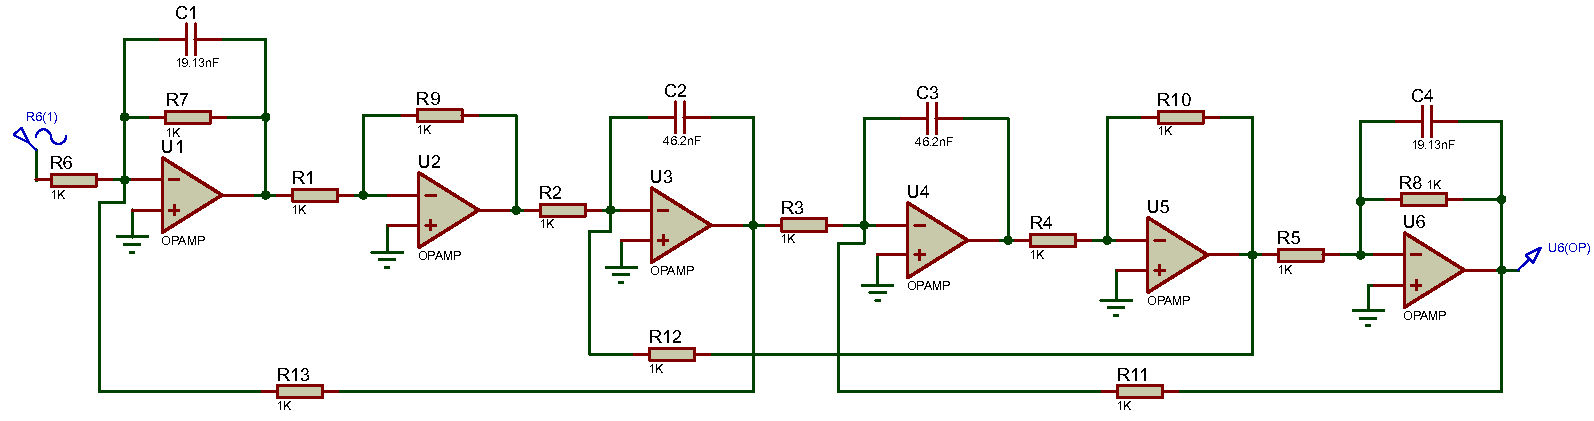
\includegraphics[width=\linewidth]{../Figures/ckt_c}
    \caption{Proteus circuit for designed lowpass filter at 40000 rad/s}
    \label{fig:protC}
\end{figure}
\proteusObservationA{protC}{0}{4.80}{lowpass filter designed in Problem 3}
\section{Discussion and Conclusion}
In this lab experiment, we dealt with active simulation of passive circuits to design higher order filters. The different methods have been discusses in brief in this report as a part of the experiment. Elemental simulation included use of FDNR and simulated inductor, both of which were realized using GIC shown in Figure~\ref{fig:gic}. The design of lowpass filter in Problem 1 was related to design using FDNR. Similarly, in Problem 2, initially the given lowpass circuit in Figure~\ref{fig:ques} was transformed into a highpass circuit shown in Figure~\ref{fig:hp}. Then GIC was used to simulate grounded inductors allowing us to design the required filter. Lastly, Problem 3 dealt with functional simulation of the ladder rather than elemental simulation. The observations for all the exercises are included in the report. Problem 1 and Problem 2 had observations that match the actual design parameters given in the problems. However, although the circuit for Problem 3 shown in Figure~\ref{fig:protC} is correct, the simulation showed some peculiar result that is included in the report.
\\
Hence, the objectives of the lab were fulfilled with the understanding of the mentioned topics.
\end{document}